\documentclass[a4paper,14pt]{extarticle}

\usepackage[top=2.5cm, bottom=2.5cm, left=2.5cm, right=2.5cm]{geometry}
\usepackage[utf8]{inputenc}
\usepackage[russian]{babel}
\usepackage[final]{graphicx}
\usepackage{caption}
\usepackage{subcaption}
\usepackage{chngcntr}
\usepackage{amsmath}
\usepackage{amsfonts}
\usepackage{pgfplots}
\usepackage{pgfplotstable}
\usepgfplotslibrary{fillbetween}
\usepackage{float}
\usepackage{lipsum}% http://ctan.org/pkg/lipsum
\usepackage{multicol}% http://ctan.org/pkg/multicol
\usepackage{hhline}
\usepackage{tabularx}
\usepackage{tikz,xcolor}
\usepackage{tkz-graph}
\usepackage{float}
\usepackage{mathtools}
\usepackage{todonotes}
\usepackage{listings}
\usepackage{epstopdf}
\usepackage{epsfig}
\usepackage[makeroom]{cancel}

\usetikzlibrary{arrows, petri, topaths}

\counterwithin{figure}{section}
\counterwithin{equation}{section}
\counterwithin{table}{section}

\DeclareMathOperator*{\argmin}{arg\,min}
\DeclareMathOperator*{\argmax}{arg\,max}
\DeclareMathOperator{\sinc}{sinc}

\definecolor{mygreen}{RGB}{28,172,0} % color values Red, Green, Blue
\definecolor{mylilas}{RGB}{170,55,241}

\lstset{language=Matlab,%
  %  basicstyle=\color{red},
    breaklines=true,%
    morekeywords={matlab2tikz,ylim,xlim,square,ones,double},
    keywordstyle=\color{blue},%
    morekeywords=[2]{1}, keywordstyle=[2]{\color{black}},
    identifierstyle=\color{black},%
    stringstyle=\color{mylilas},
    commentstyle=\color{mygreen},%
    showstringspaces=false,%without this there will be a symbol in the places where there is a space
    numbers=left,%
    numberstyle={ \color{black}},% size of the numbers
    numbersep=15pt, % this defines how far the numbers are from the text
    emph=[1]{for,end,break,switch,case,otherwise},emphstyle=[1]\color{red}, %some words to emphasise
    %emph=[2]{word1,word2}, emphstyle=[2]{style},    
}


\begin{document}
\begin{titlepage}
\centering 
{\bfseries Санкт-Петербургский Политехнический Университет} \\
Институт компьютерных наук и технологий \\
Кафедра компьютерных систем и программных технологий \\
\vspace{5cm}
{\centering \textbf{Отчёт по лабораторной работе №3} \\ 
\vspace{0.15cm}
\textbf{Дисциплина}: Телекоммуникационные технологии \\
\vspace{0.15cm}
\textbf{Тема}: Линейная фильтрация.} \\
\vspace{4cm}
\hfill {\bfseries Работу выполнил студент}  \\
\hfill гр. 33501/4 Леженин Ю.И. \\
\hfill {\bfseries Преподаватель}  \\
\hfill Богач Н.В.
\vfill
Санкт-Петербург \\
{\large \today\par}
\end{titlepage}

\section{Цель работы.}

Изучить воздействие ФНЧ на тестовый сигнал с шумом.

\section{Постановка задачи.} 

Cгенерировать гармонический сигнал с шумом
и синтезировать ФНЧ. Получить сигнал во временной и частотной
областях до и после фильтрации. Сделать выводы о воздействии
ФНЧ на спектр сигнала.

\section{Ход работы.}

Преобразование непрерывных сигналов в линейных цепях с постоянными параметрами может быть описано с помощью линейных дифференциальных уравнений с постоянными коэффициентами.

При прохождении гармонического сигнала через такую цепь меняется его амплитуда и фаза: 
\begin{equation*}
x(t) = A_x e^{j (2 \pi f t + \phi_x)} \rightarrow y(t) = A_y e^{j (2 \pi f t + \phi_y)}.
\end{equation*} 
Отношение выходного сигнала ко входному произвольной частоты называется частотной характеристикой (ЧХ):
\begin{equation*}
G(f) = \frac{A_y}{A_x} e^{j (\phi_y - \phi_x)} = |G(f)|e^{j \phi(f)}.
\end{equation*}
Модуль $|G(f)|$ называется амплитудно-частотная характеристика, $\phi(f)$ -- фазо-частотная характеристика.
Реакция цепи $g(t)$ на единичный $\delta$-импульс называется импульсная характеристика (ИХ).

При прохождении через цепь произвольного сигнала $x(t)$, спектр выходного сигнала $y(t)$ имеет вид
\begin{equation*}
Y(f) = X(f) G(f).
\end{equation*}
Согласно теореме о свертки выходной сигнал может быть найден как 
\begin{equation*}
y(t) = x(t) * g(t) = \int_{-\infty}^{t} x(t')g(t - t') dt'.
\end{equation*}   

Линейные цепи широко используются в качестве фильтров, они позволяют  изменять амплитуду гармоник на заданных частотах. 

%todo

Для демонстрации работы фильтров был смоделирован гармонический  сигнал $x(t) = sin(2\pi \, 5 t) - 0.5 cos(2\pi \, 2.5 t)$ с добавленным белым шумом. Исходный и зашумленные сигналы приведены на рисунке \ref{sig}.
 
\begin{figure}[H]
\centering
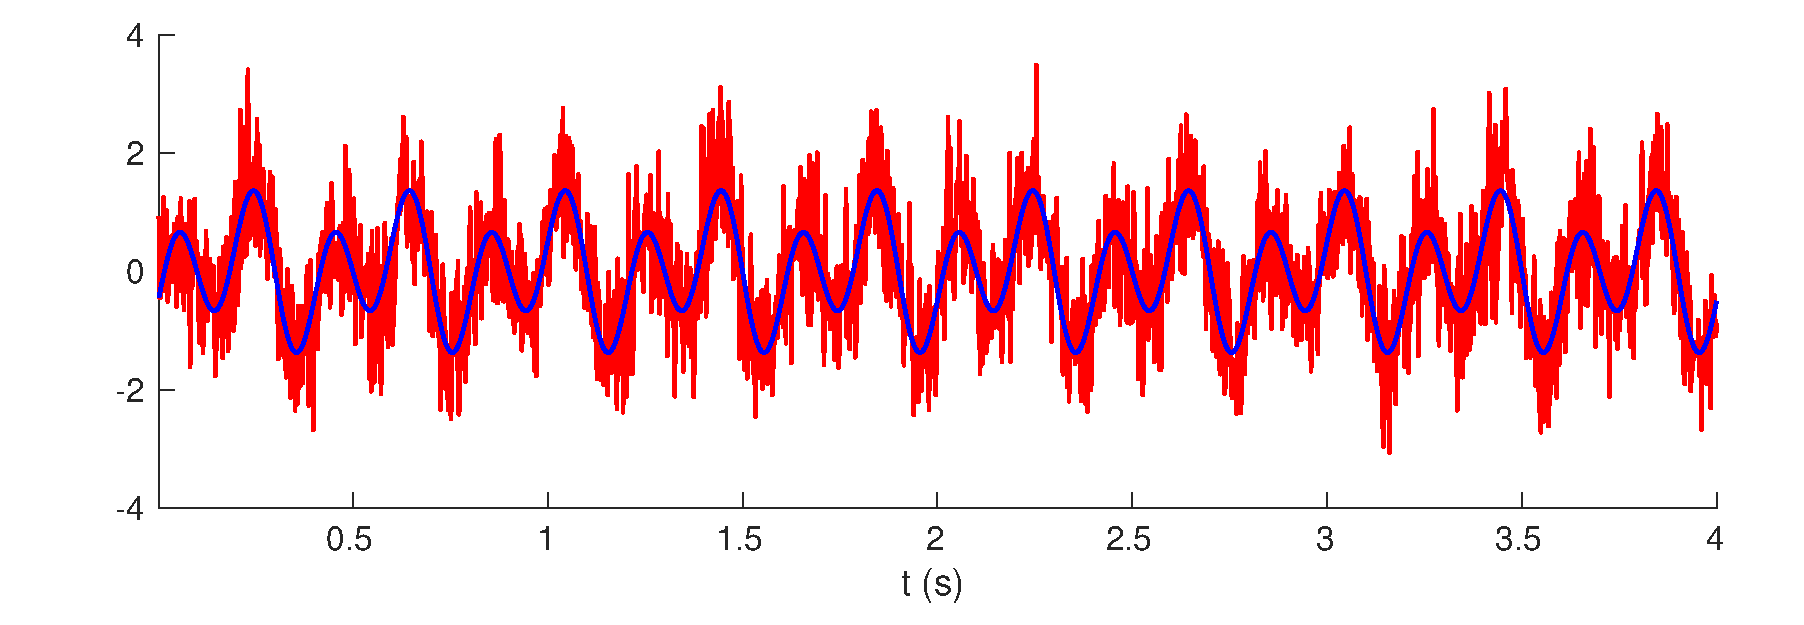
\includegraphics[width=0.95\textwidth]{./signal.eps}
\captionsetup{justification=centering,margin=1cm}
\caption{Обрабатываемый сигнал.}
\label{sig}
\end{figure}

\section{Выводы.}

%Преобразование Фурье позволяет представить сигнал в базисе гармонических колебаний разной частоты. Это значительно облегчает обработку и синтез сигналов.
%
%Важнейшими свойствами ПФ являются теорема о свертывании сигналов и теорема о перемножении сигналов: произведение функций - это свертка их образов, свертка функций - это произведение их образов.
%
%Спектр периодического сигнала дискретный, а дискретного - периодический. Если сигнал конечный, то при выполнении преобразования его образ сворачивается с функцией $\sinc(\pi f)$. 
%
%Корреляция дает возможность определить степень схожести двух сигналов, расчет с учетом смещения позволяет определить и компенсировать временные задержки. Данный инструмент часто применяется для поиска известной последовательности во входном сигнале.

\section{Приложение.}

\lstinputlisting[frame=single, caption=Программа для генерации и фильтрации сигналов.]{lab3_script.m}


\end{document}